\documentclass[14pt]{article}
\usepackage{hyperref}
\usepackage[utf8x]{inputenc}
\usepackage[english,russian]{babel}
\usepackage{cmap}
\usepackage{amsmath}
\usepackage{graphicx}
\usepackage{amssymb}
\graphicspath{ {./q1_img/} }
\usepackage[left=2cm,right=2cm,
    top=2cm,bottom=2cm,bindingoffset=0cm]{geometry}

\title{Билеты по математическому анализу для коллоквиума 14 ноября }
\author{Шишминцев Дмитрий Владимирович}

\begin{document}
    \maketitle
    \tableofcontents
    \newpage
    
    \section{Множества и операции над ними}
        \textsc{(Условно) Множество  }
         - совокупность некоторых объектов определенных по одному признаку. \\
        $ a \in A $ - элемент a принадлежит множеству A \\ 
        $ a \notin A $ - элемент a не принадлежит множеству A \\ 
        $ A \subset B $ - множество A является подмножеством B \\
        \\
        \textsc{Равенство множеств: } Множества равны если каждый элемент множества A является элементом множества B и наоборот \\
        $A = B \Leftrightarrow \begin{cases}
            x \in A \Rightarrow x \in B \\ 
            x \in B \Rightarrow x \in A
        \end{cases}$\\
        \\
        \textsc{Операции над множествами:}
        \begin{itemize}
            \item Пересечение множеств: $ A \cup B = \{ x| x \in A$ и $x \in B \}$ - коммутативно и ассоциативно
            \item Объединение множеств: $ A \cap B = \{ x | x \in A$ или $x \in B \}$ - коммутативно и ассоциативно
            \item Разность множеств: $ A \backslash B = \{ x | x \in A $и$ x \notin B \} $
            \item Симметричная разность: $ A \bigtriangleup B = (A \backslash B) \cap (B \backslash A)$
            \item Декартово произведение множеств: $ A \times B = \{(a; b) | a \in A, b \in B \}$
        \end{itemize}
           
    \section{Отображения и функции}
        \textsc{Отображение (функция) } - правило по которому $ \forall x \in A \exists ! y \in B $ \\
        \\
        Варианты функциональных отображений $F : X \rightarrow Y $
        \begin{itemize}
            \item Функция F сюръективна, если $ \forall y \in Y \exists x \in X :y = F(x)$ - каждый элемент множества Y является прообразом хотя бы одного элемента множества X
            \item Функция F инъективна, если $ \forall x \in X \exists y \in Y : y = F(x) $ - разные элементы множества X переводятся в разные элементы множества Y
            \item Функция F биективна, если она сюръективна и инъективна одновременна
        \end{itemize}
        \begin{center}
            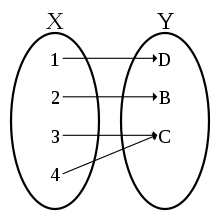
\includegraphics[scale=0.27]{2-1} 
            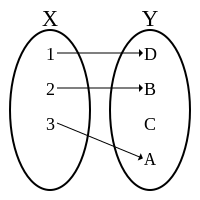
\includegraphics[scale=0.3]{2-2}
            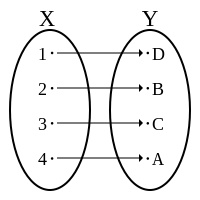
\includegraphics[scale=0.3]{2-3}    
        \end{center}
        
    \section{Эквивалентность, счетность, мощность континума}    
        \textsc{Мощность множества: } $|A|$ - число элементов входящих в множество A \\   
        \textsc{Эквивалентность множеств:} множества эквивалентны $(A \sim B)$ если $|A| = |B|$ \\
        \textsc{Счетность множество: } бесконечное множество, элементы которого можно пронумеровать натуральными числами \\
        \textsc{Мощность континуума: } мощность множества всех вещественных чисел 
 
    \section{Теорема Кантора-Бернштейна и сравнение мощности множеств}  
        \textsc{Теорема Кантора-Бернштейна} 
        \begin{enumerate}
            \item Если $A \sim B'$ (где $B' \subset B$) и $B \sim A'$ ( где $A' \subset A $) $\rightarrow A \sim B$    
            \item Если $A \subset B \subset C$, причем $A \sim C$, то $A \sim B$
        \end{enumerate}
        \textsc{Сравнение мощностей множеств:} Если множества $A$ и $B$ неэквивалентны, но $\exists B' \subset B: B' \sim A $ и $\nexists  A' \subset A: A' \sim B$, то будем считать, что $|A|<|B|$

    \section{Множество вещественных чисел и его аксиоматика}
        \textsc{Вещественные числа $\mathbb{R}$:} бесконечные десятичные дроби вида $\pm a_0,a_1a_2a_3....$, где выбран определенный знак: + или -, $a_0 \in \mathbb{N} \cup \{0\}$, а все десятичные символы $a_1, a_2...$ - цифры от 0 до 9, т.е. $\forall n \in \mathbb{N} \rightarrow a_n \in \{0,1,2,...,9\}$
        \textsc{Аксиоматика: }
            \begin{enumerate}
                \item Линейность: если $x \neq y$, то $x > y$ или $x < y$
                \item Транзитивность: $\exists\{ >,= \}b, b\{ >,= \}c\rightarrow a\{>,=\}c$
                \item Ассоциативность: $\forall a, b, c \in \mathbb{R} \rightarrow (a+b)+c = a+(b+c), a(bc) = (ab)c$
                \item Коммутативность: $\forall a,b \in \mathbb{R} \rightarrow a+b=b+a, a\cdot b = b\cdot a $
                \item Дистрибутивность: $\forall a,b,c \in \mathbb{R} \rightarrow (a+b)\cdot c = a \cdot c + b \cdot c$
            \end{enumerate}

    \section{Ограниченность множества и его точные грани}  
        \textsc{Непустое множество $A \subset \mathbb{R}$ называется:} \\
        \begin{enumerate}
            \item Ограниченным сверху, если $\exists b \in \mathbb{R}: \forall a \in A \rightarrow a \leqslant  b$
            \item Ограниченным снизу, если $\exists d \in \mathbb{R}: \forall a \in A \rightarrow d \leqslant  a$
            \item Ограниченным, если $\exists c \in \mathbb{R}: c>0$ и $\forall a \in A \rightarrow |a| \leqslant c$
        \end{enumerate}
        Верхняя и нижняя грань не единственны. \\
        \textsc{Свойство точной верхней грани:} Если $b = sup A $, то $\forall \epsilon > 0 \exists a \in A: a > b - \epsilon$ \\
        \textsc{Свойство точной нижней грани:} Если $d = inf A $, то $\forall \epsilon > 0 \exists a \in A: a < d + \epsilon$

    \section{Метод математической индукции}
        \textsc{Математическая индукция } - метод математического доказательства, который используется, чтобы доказать истинность некоторого утверждения для всех натуральных чисел.
        Для обоснования метода математической индукции используется свойство натуральных чисел:  $\forall A \subset \mathbb{N}: A \ne \emptyset \exists a' \in A : \forall a \in A \rightarrow a' \leqslant a$ \\ 

        Метод математической индукции состоит из следующих шагов:
        \begin{enumerate}
            \item База индукции: проверяем справедливость утверждения для a'
            \item Индукционное предположение: предполагаем справедливость для произвольного элемента $a_k \in A$
            \item Индукционный шаг: доказываем справедливость утверждения для $a_{k+1} \in A$
        \end{enumerate}

    \section{Бином Ньютона}
        $(1+x)^n = \sum^n_{k=0} C^k_n x^k$, где $C^k_n = 
        \begin{pmatrix}
            n \\ k
        \end{pmatrix} 
        = \frac{n!}{k!(n-k)!}$ - биноминальный коэффициент, $n,k \in \mathbb{N}, x \in \mathbb{R}$

    \section{Числовая последовательность и ее ограниченность}
        \textsc{Числовая последовательность:} функция определенная на множестве $\mathbb{N}$ и принимающая числовые значения. $\exists x_n = f(n)$, где $f:\mathbb{N} \rightarrow  \mathbb{R}$, тогда $\{x_n \}$ - последовательность \\
        \textsc{Ограниченность последовательности: } последовательность называется ограниченной с обеих сторон, если $\exists A \in \mathbb{R}: \forall n \in \mathbb{N} \rightarrow |x_n| \leqslant A$

    \section{Бесконечно большие и бесконечно малые последовательности и их связь}
        \textsc{Бесконечно большая последовательность: } $\forall c > 0 \exists n(c) \in \mathbb{N} : \forall n > n(c) \rightarrow |x_n| > c$ \\ 
        \textsc{Бесконечно малая последовательность: } $\forall \epsilon > 0 \exists n(\epsilon) \in \mathbb{N} : \forall n > n(\epsilon) \rightarrow |x_n| < \epsilon$ \\
        \textsc{Связь:} если $\{x_n\}$ - б.м.п. и $\forall n \in \mathbb{N} \rightarrow x_n \ne 0 $, то $\{\frac{1}{x_n}\}$ - б.б.п и наоборот, \\ если $\{x_n\}$ - б.б.п. и $\forall n \in \mathbb{N} \rightarrow x_n \ne 0 $, то $\{\frac{1}{x_n}\}$ - б.м.п и наоборот,
    
    \section{Сходимость и расходимость последовательностей}
        \textsc{Определение} - Последовательность $\{x_n\}$ называется сходящейся (имеющей предел), если: \\ $\forall \epsilon > 0 \exists n(\epsilon) \in \mathbb{N}: \forall n > n(\epsilon) \rightarrow |x_n - a| < \epsilon$ \\
        \textsc{Определение} - Последовательность $\{x_n\}$ называется сходящейся (имеющей предел), если: \\ $\forall \epsilon > 0 \exists n(\epsilon) \in \mathbb{N}: \forall n > n(\epsilon) \rightarrow x_n \in \mathbb{U}_{\epsilon} (a)$ \\
        Последовательности не являющиеся сходящими, принято называть расходящимися. \\
        \textsc{Определение} - Последовательность $\{x_n\}$ называется сходящейся (имеющей предел), если: $\exists a \in \mathbb{R}\ \backslash \{ \pm \infty \}: a_n$ является б.м.п, где $a_n := x_n - a$ \\
        Если $\{x_n\}$ сходиться, то она имеет единственный предел.


\end{document}